%\documentclass[handout]{beamer} % Sin animaciones
% https://tex.stackexchange.com/questions/74805/latex-error-option-clash-for-package-xcolor
\documentclass[xcolor={dvipsnames},spanish]{beamer}
%\usetheme{Warsaw}
\usetheme{Madrid}
\setbeamertemplate{navigation symbols}{} % remove navigation symbols
%\setbeamercolor{alerted text}{fg=orange}

\usepackage{thesis}
\usepackage{sections/nd_rules}
\setbeamertemplate{footline}[frame number]

% https://tex.stackexchange.com/questions/464916/listing-inside-a-frame-using-beamer
\lstset{language=ppa, xleftmargin=0.5cm}

\renewcommand{\lstlistingname}{Programa}

\usepackage{fitch}

% https://tex.stackexchange.com/questions/178800/creating-sections-each-with-title-pages-in-beamers-slides
\AtBeginSection[]{
  \begin{frame}
  \vfill
  \centering
  \begin{beamercolorbox}[sep=8pt,center,shadow=true,rounded=true]{title}
    \usebeamerfont{title}\insertsectionhead\par%
  \end{beamercolorbox}
  \vfill
  \end{frame}
}

\newenvironment{command}
    {
        \begin{beamercolorbox}[sep=8pt,center,shadow=true,rounded=true]{block body}
    }
    {\end{beamercolorbox}}


% Justificaciones
\newcommand{\just}[1]{\textcolor{violet}{(#1)}}

% Tiempo total para dar la presentación: 60 minutos, 15 para preguntas

% Notas

\title{PPA}
\subtitle{Un asistente de demostración para
lógica de primer orden con extracción de
testigos usando la traducción de Friedman}
\author{Manuel Panichelli}
\institute{Deparatamento de Computación, FCEyN, UBA}
\date{Diciembre 2024}

\begin{document}


\frame{\titlepage}

\section{Introducción}

% TODO: Considerar explicar que es un teorema y qué es la verificación
\begin{frame}{Asistentes de demostración}
    \begin{itemize}
        \item Los \textbf{asistentes de demostración} son herramientas que
        facilitan la escritura y el chequeo de demostraciones por
        computadora.
        \item Usos usuales: formalización de teoremas matemáticos y verificación de programas.
        \item Ventajas:\footnote{\href{https://youtu.be/AayZuuDDKP0?si=eGETzgh9PQ_8JecR}{Terrence Tao - Machine Assisted Proof}}
        \begin{itemize}
            \item Facilitan la colaboración a gran escala (mediante la confianza en el asistente).
            \item Habilitan generación automática de demostraciones con IA. Por ej. un \textit{LLM} (como \textit{ChatGPT}) suele devolver alucinaciones, que pueden ser filtradas automáticamente con un asistente.
        \end{itemize}
    \end{itemize}
\end{frame}

\begin{frame}{Asistentes de demostración}
    Implementan distintas \textit{teorías}. \todo{No me gusta teoria, se usa
    para teorias de primer orden}
    Ejemplos:
    \begin{itemize}
        \item Mizar (lógica de primer orden)
        \item Coq (teoría de tipos)
        \item Agda (teoría de tipos)
        \item Isabelle (lógica de orden superior / teoría de conjuntos ZF)
    \end{itemize}
\end{frame}

\begin{frame}{PPA}
    \begin{itemize}
        \item Diseñamos e implementamos \textbf{PPA} (\textit{Pani's Proof
        Assistant}), un asistente de demostración para lógica \textbf{clásica}
        de primer orden.
        \item Permite hacer extracción de testigos: dada una demostración de
        $\exists \var . \pred(\var)$, encuentra $\term$ tal que $\pred(\term)$.
        \item Aporte principal: implementación de extracción de testigos para lógica clásica de forma directa (vemos los detalles después).
    \end{itemize}
    
\end{frame}

\begin{frame}{Representación de demostraciones}
    Queremos escribir demostraciones en la computadora. ¿Cómo las representamos?. Veamos un ejemplo.
    
    \begin{itemize}
        \item Tenemos dos premisas
        \begin{enumerate}
            \item Los alumnos que faltan a los exámenes, los reprueban.
            \item Si se reprueba un final, se recursa la materia.
        \end{enumerate}
        \item A partir de ellas, podríamos demostrar que si un alumno falta a un final, entonces recursa la materia.
    \end{itemize}

    \begin{block}{Teorema}
        Si ((falta entonces reprueba) y (reprueba entonces recursa)) y falta, entonces recursa
    \end{block}
    \begin{exampleblock}{Demostración}
        \begin{itemize}
    \item Asumo que falta. Quiero ver que recursa.
    \item Sabemos que si falta, entonces reprueba. Por lo tanto reprobó.
    \item Sabemos que si reprueba, entonces recursa. Por lo tanto recursó. \qed
\end{itemize}
    \end{exampleblock}
\end{frame}

\begin{frame}{Sistemas deductivos}
    \begin{itemize}
        \item La demostración anterior es poco precisa. No se puede representar rigurosamente.
        \item Necesitamos \textbf{sistemas deductivos}: sistemas lógicos formales usados para demostrar setencias. Pueden ser representados como un tipo abstracto de datos.
        \item Usamos \textbf{deducción natural}. Compuesto por,
        \begin{itemize}
            \item \textbf{Lenguaje formal}: lógica de primer orden.
            \item \textbf{Reglas de inferencia}: lista de reglas que se usan para probar teoremas a partir de axiomas y otros teoremas. Por ejemplo, \textit{modus ponens} (si
    es cierto $\form \fImp \formTwo$ y $\form$, se puede concluir $\formTwo$) o
    \textit{modus tollens} (si es cierto $\form \fImp \formTwo$ y $\fNot
    \formTwo$, se puede concluir $\fNot\form$)
    \item \textbf{Axiomas}: fórmulas de $L$ que se asumen válidas. Todos los
    teoremas se derivan de axiomas. Se usan para modelar \textit{teorías} de
    primer orden (por ej. teoría de estudiantes en la facultad).
        \end{itemize}
    \end{itemize}
\end{frame}

\begin{frame}{Lógica de primer orden}

\begin{definition}[Términos]
    Los términos están dados por la gramática:
    \begin{align*}
        \term ::= &\ \var                               &\text{(variables)} \\
                  & \mid \fun(\term_1, \dots, \term_n) &\text{(funciones)}
    \end{align*}
\end{definition}
\begin{definition}[Fórmulas]
    Las fórmulas están dadas por la gramática:
    \begin{align*}
        \form, \formTwo ::=
         & \ \pred(\term_1, \dots, \term_n) & (\text{predicados})                \\
         & \mid \fFalse                     
           \mid \fTrue                      & \text{(falso o \textit{bottom} y verdadero o \textit{top})} \\
         & \mid \form \fAnd \formTwo                        
           \mid \form \fOr \formTwo           & \text{(conjunción y disyunción)}     \\
         & \mid \form \fImp \formTwo                       
           \mid \fNot \form                 & \text{(implicación y negación)}                  \\
         & \mid \forall \var . \form        
           \mid \exists \var . \form        & \text{(cuantificador universal y existencial)}
    \end{align*}
\end{definition}

\end{frame}

% \begin{frame}{Lógica de primer orden}
% Los predicados son \textbf{fórmulas atómicas}. Los de aridad 0 además son llamados \textit{variables proposicionales}.

% \begin{notation*}
%     Usamos
%     \begin{itemize}
%         \item $\var, \varTwo, \varThree, \dots$ como \textbf{variables}.
%         \item $\fun, \funTwo, \funThree, \dots$ como \textbf{símbolos de función}.
%         \item $\pred, \predTwo, \predThree, \dots$ como \textbf{símbolos de predicado}.
%         \item $\term, \termTwo, \dots$ para referirnos a \textbf{términos}.
%         \item $\formLit, \formLitTwo, \formLitThree, \dots$, $\form, \formTwo, \formThree, \dots$ y $\anyForm, \anyFormTwo, \dots$ para referirnos a \textbf{fórmulas}.
%     \end{itemize}
% \end{notation*}
% \end{frame}

\section{Deducción natural}

\begin{frame}{Deducción natural}
    \begin{definitions}
        \begin{itemize}
            \item $\ctx$ es un \textbf{contexto de demostración}, conjunto de
            fórmulas que se asumen válidas
            \item Notación: $\ctx, \anyForm = \ctx \cup \{\anyForm\}$
            \item $\judG$ es la \textbf{relación de derivabilidad} definida a
            partir de las \textit{reglas de inferencia}. Permite escribir
            juicios $\ctx \judG \anyForm$.
            \item Intuición: \textit{``$\anyForm$ es
            una consecuencia de las suposiciones de $\ctx$''}
            \item El juicio es cierto si en una cantidad finita de
            pasos podemos concluir $\anyForm$ a partir de las fórmulas de
            $\ctx$, los axiomas y las reglas de inferencia.
            \item Decimos que
            $\anyForm$ es \textit{derivable} a partir de $\ctx$.
        \end{itemize}
    \end{definitions}
\end{frame}

\begin{frame}{Reglas de inferencia}
    \begin{definition}[Reglas de inferencia]
        \begin{columns}
            \column{0.5\textwidth}
            \proofTreeAx
            \proofTreeImpI
            \proofTreeImpE
            \column{0.5\textwidth}
            \proofTreeAndI
            \proofTreeAndEOne
            \proofTreeAndETwo
        \end{columns}
        
    \end{definition}
    Dos tipos para cada conectivo y cuantificador, dada una fórmula formada con un conectivo:
    \begin{itemize}
        \item \textbf{Introducción}: ¿Cómo la demuestro?
        \item \textbf{Eliminación}: ¿Cómo la uso para demostrar otra?
    \end{itemize}
\end{frame}

\begin{frame}{Ejemplo}
    Vamos a demostrar el ejemplo informal en deducción natural. Lo modelamos
    para un alumno y materia particulares. Notamos:
    \begin{itemize}
        \item $\reprueba \equiv \predReprueba(juan, \funFinal(logica))$
        \item $\recursa \equiv \predRecursa(juan, logica)$
        \item $\falta \equiv \predFalta(juan, \funFinal(logica))$
    \end{itemize}

    Queremos probar entonces 
    \[
        \Big(
            (\falta \fImp \reprueba) \wedge (\reprueba \fImp \recursa)
        \Big)
        \fImp
        (\falta \fImp \recursa)
    \]
\end{frame}

\begin{frame}{Ejemplo}
    \begin{prooftree}
        \AxiomC{}
        \RL{\ruleAx}
        \UnaryInfC{$\ctx \judG (\falta \fImp \reprueba) \wedge (\reprueba \fImp \recursa)$}
        \RL{\ruleAndEOne}
        \UnaryInfC{$\ctx \judG \reprueba \fImp \recursa$}
        
        \AxiomC{$\someProof$}
        \noLine
        \UnaryInfC{$\ctx \judG \reprueba$}
        \RL{\ruleImpE}
        \BinaryInfC{\(
            \ctx =
            (\falta \fImp \reprueba) \wedge (\reprueba \fImp \recursa),\
            \falta
            \judG
            \recursa
        \)}
        \RL{\ruleImpI}
        \UnaryInfC{\(
            (\falta \fImp \reprueba) \wedge (\reprueba \fImp \recursa)
            \judG
            \falta \fImp \recursa 
        \)}
        \RL{\ruleImpI}
        \UnaryInfC{\(
            \judG
            \Big(
                (\falta \fImp \reprueba) \wedge (\reprueba \fImp \recursa)
            \Big)
            \fImp
            (\falta \fImp \recursa)
        \)}
    \end{prooftree}

    donde

    \begin{prooftree}
        \AxiomC{}
        \RL{\ruleAx}
        \UnaryInfC{$\ctx \judG (\falta \fImp \reprueba) \wedge (\reprueba \fImp \recursa)$}
        \RL{\ruleAndETwo}
        \UnaryInfC{$\ctx \judG \falta \fImp \reprueba$}
        \AxiomC{}
        \RL{\ruleAx}
        \UnaryInfC{$\ctx \judG \falta$}
        \RL{\ruleImpE}
        \LL{$\someProof=$}
        \BinaryInfC{$\ctx \judG \reprueba$}
    \end{prooftree}
\end{frame}

\begin{frame}{Reglas de inferencia}
    \begin{definition}[Reglas de inferencia]
        \proofTreeLEM
        \begin{columns}
            \begin{column}{0.5\textwidth}
                \proofTreeFalseE
                \proofTreeTrueI
            \end{column}
            \begin{column}{0.5\textwidth}
                \proofTreeNotI
                \proofTreeNotE
            \end{column}
        \end{columns}
        \begin{columns}
            \begin{column}{0.5\textwidth}
                \proofTreeOrIOne
            \end{column}
            \begin{column}{0.5\textwidth}
                \proofTreeOrITwo
            \end{column}
        \end{columns}
        \proofTreeOrE
    \end{definition}
\end{frame}

\begin{frame}{Reglas de inferencia}
    \begin{definition}[Sustitución]
        Notamos como $\form \subst{\var}{\term}$ a la sustitución de todas las
        ocurrencias libres de la variable $\var$ por el término $\term$ en la
        fórmula $\form$.
    \end{definition}
    \begin{definition}[Reglas de cuantificadores]
        \begin{columns}
            \column{0.5\textwidth}
            \proofTreeForallI
            \column{0.5\textwidth}
            \proofTreeForallE
        \end{columns}
        \proofTreeExistsI
        \proofTreeExistsE
    \end{definition}
\end{frame}

\begin{frame}{Reglas admisibles}
    \begin{itemize}
        \item Mencionamos \textit{modus tollens} pero no aparece en las reglas de inferencia.
        \item Queremos un sistema lógico \textbf{minimal}: no agregamos como
        regla de inferencia lo que podemos derivar a partir de las existentes,
        las reglas \textbf{admisibles}.
        \item Se implementan como \textit{macros}: cada uso de la regla
        admisible se reemplaza por su demostración.
    \end{itemize} 

    \begin{lemma}[Modus tollens]
        
    \begin{prooftree}
        \AxiomC{}
        \RL{\ruleAx}
        \UnaryInfC{\(\ctx \judG (\form \fImp \formTwo) \fAnd \fNot \formTwo\)}
        \RL{\ruleAndETwo}
        \UnaryInfC{\(
            \ctx \judG \fNot \formTwo
        \)}
        \AxiomC{}
        \RL{\ruleAx}
        \UnaryInfC{\(\ctx \judG (\form \fImp \formTwo) \fAnd \fNot \formTwo\)}
        \RL{\ruleAndEOne}
        \UnaryInfC{$\ctx \judG \form \fImp \formTwo$}
        \AxiomC{}
        \RL{\ruleAx}
        \UnaryInfC{$\ctx \judG \form$}
        \RL{\ruleImpE}
        \BinaryInfC{\(
            \ctx \judG \formTwo
        \)}
        \RL{\ruleNotE{}}
        \BinaryInfC{\(
            \ctx = (\form \fImp \formTwo) \fAnd \fNot \formTwo, \form
            \judG
            \fFalse
        \)}
        \RL{\ruleNotI{}}
        \UnaryInfC{\(
            (\form \fImp \formTwo) \fAnd \fNot \formTwo
            \judG
            \fNot \form
        \)}
        \RL{\ruleImpI{}}
        \UnaryInfC{\(\judG
            (\form \fImp \formTwo \fAnd \fNot \formTwo)
            \fImp \fNot\form
        \)}
    \end{prooftree}
    \end{lemma}
\end{frame}

\begin{frame}{Sustitución sin capturas}
    Para la sustitución $\form \subst{\var}{\term}$ queremos evitar la
    \textbf{captura de variables}, por ejemplo
    \[
        (\forall \varTwo . \pred(\var))\subst{\var}{\varTwo} \overset{?}{=}
        \forall \varTwo . \pred(\alert{\varTwo})
    \]
    sustituyendo sin más, capturamos a la variable $\var$ que ahora está ligada.
    Lo evitamos \textbf{automáticamente}: cuando se encuentra con una captura,
    se renombra la variable ligada de forma que no ocurra
    \[
        (\forall \varTwo . \pred(\var))\subst{\var}{\varTwo} =
        \forall \alert{\varThree} . \pred(\varTwo)
    \]
\end{frame}

\begin{frame}{Alfa equivalencia}
    \begin{itemize}    
        \item Si tenemos una hipótesis $\exists \var . \pred(\var)$ queremos poder
        usarla para demostrar $\exists \varTwo . \pred(\varTwo)$.
        \item No son iguales, pero son \textbf{\bm{$\alpha$}-equivalentes}: si
        renombramos variables ligadas de forma apropiada, son iguales.
        \item Algoritmo naíf: cuadrático en la estructura de la fórmula,
        renombrando recursivamente.
        \item Algoritmo cuasilineal: manteniendo dos sustituciones, una por
        fórmula.
    \end{itemize}
    \begin{example}
        \begin{align*}
            (\exists \var . \fun(\var)) &\alphaEq (\exists \varTwo . \fun(\varTwo))
            &&\{\}, \{\}
            \\
            &\iff \fun(\var) \alphaEq \fun(\varTwo)
                &&\{\var \mapsto \varThree\}, \{\varTwo \mapsto \varThree\}\\
            &\iff \var \alphaEq \varTwo
                &&\{\var \mapsto \varThree\}, \{\varTwo \mapsto \varThree\}\\
            &\iff \varThree = \varThree.
        \end{align*}        
    \end{example}
\end{frame}

\section{PPA}

\begin{frame}{Mathematical vernacular}
    Aparentemente hay una forma canónica de presentar demostraciones matemáticas\footnote{\textit{Mathematical
    Vernacular} de Freek Wiedijk}. Descubierta e implementada independientemente en Mizar,
    Isar (Isabelle), etc. Combinación de ideas:

    \begin{itemize}
        \item \textbf{Deducción natural en estilo de \textit{Fitch}}. Notación
        equivalente en la cual las demostraciones son
        representadas como listas de fórmulas en lugar de árboles. Las que
        aparecen antes justifican las que aparecen después.
        \item \textbf{Reglas de inferencia \textit{declarativas}}: una forma de afirmar
        que $\form_1, \dots, \form_n \judG \form$ es válida, sin
        tener que demostrarlo a mano.
        \item \textbf{Sintaxis similar a un lenguaje de programación} en lugar del
        lenguaje natural usado para demostraciones.
    \end{itemize}
\end{frame}

\begin{frame}[fragile]{PPA}
    Diseñamos e implementamos el \textit{lenguaje} PPA, inspirado en el
    \textit{mathematical vernacular}. Veamos la \textbf{interfaz} completa y luego la implementación.
    \lstinputlisting[title=Ejemplo demostración]{listings/ppt/alumnos-corto.ppa}
\end{frame}

\begin{frame}[fragile]{Programas}
    Un \textbf{programa} de PPA consiste en una lista de \textbf{declaraciones},
    que pueden ser
    \begin{itemize}
        \item \textbf{Axiomas}: fórmulas que se asumen válidas
        \begin{lstlisting}[numbers=none]
axiom <name> : <form>
        \end{lstlisting}
        \item \textbf{Teoremas}: fórmulas junto con sus demostraciones.
\begin{lstlisting}[numbers=none]
theorem <name> : <form>
proof
    <steps>
end
\end{lstlisting}
    \end{itemize}
\end{frame}

\begin{frame}[fragile]{Identificadores}
    \begin{itemize}
        \item \textbf{Variables} (\lstinline{<var>})
        \begin{center}
            \verb/(\_|[A-Z])[a-zA-Z0-9\_\-]*(\')*/
        \end{center}
        \item \textbf{Identificadores} (\lstinline{<id>})
        \begin{center}
            \verb/[a-zA-Z0-9\_\-\?!#\$\%\*\+\<\>\=\?\@\^]+(\')*/
        \end{center}
        \item \textbf{Nombres} (\lstinline{<name>})
        
        Pueden ser identificadores o strings arbitrarios encerrados por comillas dobles.
        \begin{center}
            \verb/<id> | \"[^\"]*\"/
        \end{center}
    \end{itemize}
\end{frame}

\begin{frame}[fragile]{Fórmulas y términos}
    Términos:
    \begin{itemize}
        \item Variables: \lstinline{<var>}
        \item Funciones: \lstinline{<id>(<term>, ..., <term>)}
    \end{itemize}

    Funciones:
    \begin{itemize}
        \item Predicados: \lstinline{<id>(<term>, ..., <term>)}
        \item \lstinline{<form> & <form>}
        \item \lstinline{<form> | <form>}
        \item \lstinline{<form> -> <form>}
        \item \lstinline{<form> <-> <form>}
        \item \lstinline{~ <form>}
        \item \lstinline{exists <var> . <form>}
        \item \lstinline{forall <var> . <form>}
        \item \lstinline{true}, \lstinline{false}
        \item \lstinline{(<form>)}
    \end{itemize}
\end{frame}

\begin{frame}{Demostraciones}
    \begin{itemize}
        \item Lista de comandos que reducen sucesivamente la \textit{tesis}
        (fórmula a demostrar) hasta agotarla por completo.
        \item Corresponden aproximadamente a reglas de inferencia de deducción
        natural (vistas como una demostración en el estilo de Fitch).
        \item Tienen disponible un \textbf{contexto} con todas las hipótesis
        asumidas (como axiomas) o demostradas (teoremas y comandos que
        demuestran hipótesis auxiliares).
    \end{itemize}
\end{frame}

\begin{frame}{by - El mecanismo principal de demostración}
    \begin{itemize}
        \item \lstinline{<form> by <h1>, ..., <hn>} afirma que la fórmula es una consecuencia lógica de las fórmulas que corresponden a las hipótesis provistas.
        \item Los nombres de las hipótesis son del tipo \lstinline{<name>} (o bien identificadores o \textit{strings} arbitrarios).
        \item Por debajo usa un \textit{solver} completo para lógica proposicional pero heurístico para primer órden.
        \item Se usa para eliminar implicaciones y universales.
        \item Usado por dos comandos principales: \lstinline{thus} y \lstinline{have}.
    \end{itemize}
\end{frame}


\begin{frame}[fragile]{Thus}
    \begin{command}
    \lstinline{thus <form> by <h1>, ..., <hn>}
    \end{command}

    Si \lstinline{<form>} es \textit{parte} de la tesis, y el \textit{solver} puede demostrar la implicación, lo demuestra automáticamente y lo descarga de la tesis.
    \begin{columns}
        \begin{column}{0.5\textwidth}
            \lstinputlisting[title=Eliminación de implicación]{listings/interfaz/by-imp.ppa}
        \end{column}
        \begin{column}{0.5\textwidth}
            \lstinputlisting[title=Eliminación de universal]{listings/interfaz/by-forall.ppa}
        \end{column}
    \end{columns}
\end{frame}

\begin{frame}[fragile]{Have}
    \begin{command}
    \lstinline{have <name>: <form> by <h1>, ..., <hn>}
    \end{command}

    Análogo a \lstinline{thus}, pero introduce una afirmación \textit{auxiliar}
    sin reducir la tesis, agregándola al contexto.
    
    \begin{figure}[H]
        \centering
        \small Eliminación de implicación en dos pasos
        
        \begin{tabular}{c}
            \lstinputlisting{listings/interfaz/by-imp-have.ppa}
        \end{tabular}
    \end{figure}

\end{frame}

\begin{frame}[fragile]{Hipótesis anterior}
    Ambas pueden referirse a la hipótesis anterior con guión medio
    (\lstinline{-}), y pueden hacerlo implícitamente usando \lstinline{hence} y
    \lstinline{have}.

    \begin{table}[H]
        \centering
    \begin{tabular}{l|l|l}
    Comando             & Alternativo             & ¿Reduce la tesis? \\
    \hline
    \lstinline|thus|    & \lstinline|hence|       & Sí               \\
    \lstinline|have|    & \lstinline|then|        & No              
    \end{tabular}
    \end{table}

    \begin{columns}
        \begin{column}{0.5\textwidth}
        \lstinputlisting[
            firstline=1,
            lastline=9,
            title=Eliminación en dos pasos,
        ]{listings/interfaz/by-imp-then.ppa}
        \end{column}
        \begin{column}{0.5\textwidth}
            \lstinputlisting[
                linerange={12-16, 19-23},
                numbers=none,
                title=Alternativas equivalentes,
            ]{listings/interfaz/by-imp-then.ppa}
        \end{column}
    \end{columns}
\end{frame}

\begin{frame}[fragile]{By opcional}
    \begin{itemize}
        \item El \lstinline{by} es opcional
        \item Si se omite, la fórmula debe ser
        demostrable por el \textit{solver} sin partir de ninguna hipótesis
        \item Vale para todas las tautologías proposicionales.
    \end{itemize}

    \begin{figure}[H]
        \centering
        \small Tautología proposicional
        
        \begin{tabular}{c}
            \lstinputlisting{listings/interfaz/by-taut.ppa}
        \end{tabular}
    \end{figure}
\end{frame}

\begin{frame}{Comandos y reglas de inferencia}
    \begin{columns}
        \begin{column}{0.5\textwidth}
            \begin{table}[H]
                \centering
                \begin{tabular}{c|c}
                Regla & Comando \\
                \hline
                \ruleLEM        &   \lstinline|cases| \\
                \ruleAx         &   \lstinline|by| \\
                \ruleExistsI    &   \lstinline|take| \\
                \ruleExistsE    &   \lstinline|consider| \\
                \ruleForallI    &   \lstinline|let| \\
                \ruleForallE    &   \lstinline|by| \\
                \ruleOrIOne     &   \lstinline|by| \\
                \ruleOrITwo     &   \lstinline|by| \\
                \ruleOrE        &   \lstinline|cases|
                \end{tabular}
            \end{table}
        \end{column}
        \begin{column}{0.5\textwidth}
            \begin{table}[H]
                \centering
                \begin{tabular}{c|c}
                Regla & Comando \\
                \hline
                \ruleAndI       &   \lstinline|by| \\
                \ruleAndEOne    &   \lstinline|by| \\
                \ruleAndETwo    &   \lstinline|by| \\
                \ruleImpI       &   \lstinline|suppose| \\
                \ruleImpE       &   \lstinline|by| \\
                \ruleNotI       &   \lstinline|suppose| \\
                \ruleNotE       &   \lstinline|by| \\
                \ruleTrueI      &   \lstinline|by| \\
                \ruleFalseE     &   \lstinline|by|
                \end{tabular}
            \end{table}
        \end{column}
    \end{columns}
\end{frame}

\begin{frame}[fragile]{Suppose (\ruleImpI / \ruleNotI)}
    \begin{command}
        \lstinline{suppose <name>: <form>} \quad (\ruleImpI / \ruleNotI)
    \end{command}

    \begin{itemize}
        \item  Si la tesis es una implicación $\form \fImp \formTwo$, agrega el antecedente
        $\form$ como hipótesis con el nombre dado y reduce la tesis al consecuente
        $\formTwo$
        \item Viendo la negación como una implicación $\fNot \form \equiv
        \form \fImp \fFalse$, permite introducir negaciones, tomando
        $\formTwo = \fFalse$.
    \end{itemize}

    \begin{columns}
        \begin{column}{0.5\textwidth}
            \lstinputlisting[
                firstline=1, lastline=7,
                title=Introducción de implicación,
            ]{listings/interfaz/suppose.ppa}
        \end{column}
        \begin{column}{0.5\textwidth}
            \lstinputlisting[
                firstline=9, lastline=15,
                title=Introducción de negación,
            ]{listings/interfaz/suppose.ppa}    
        \end{column}
    \end{columns}
\end{frame}

\begin{frame}[fragile]{Cases (\ruleOrE)}
    \begin{command}
        \lstinline{cases by <h1>, ..., <hn>} \quad (\ruleImpI / \ruleNotI)
    \end{command}
    \begin{columns}
        \begin{column}{0.5\textwidth}
        \begin{itemize}
            \item Permite razonar por casos a partir de una disyunción. Para cada uno, se debe
            demostrar la tesis en su totalidad.
            \item Si los casos son \lstinline{<f1>} a
            \lstinline{<fn>}, tiene que valer \lstinline{<f1> | ... | <fn> by} \lstinline{<h1>, ..., <hn>}.
            \item Se puede omitir el \lstinline{by} para razonar mediante LEM (casos $\anyForm$ y $\fNot \anyForm$).
        \end{itemize}
        \end{column}
        \begin{column}{0.5\textwidth}
            \lstinputlisting[
        title=Cases,
        firstline=1, lastline=11,
    ]{listings/interfaz/cases.ppa}
        \end{column}
    \end{columns}
\end{frame}

\begin{frame}[fragile]{Take (\ruleExistsI)}
    \begin{command}
        \lstinline{take <var> := <term>} \quad (\ruleExistsI)
    \end{command}
    \vfill
    \begin{itemize}
        \item Introduce un existencial instanciando su variable y reemplazándola por un término.
        \item Si la tesis es \lstinline{exists X . p(X)}, luego de \lstinline{take X := a}, se reduce a \lstinline{p(a)}.
    \end{itemize}
\end{frame}

\begin{frame}[fragile]{Consider (\ruleExistsE)}
    \begin{command}
        \lstinline{consider <var> st <name>: <form> by <h1>, ..., <hn>} \quad (\ruleExistsE)
    \end{command}
    \begin{itemize}
        \item Si se puede justificar \lstinline{exists X. p(X)}, permite razonar sobre tal \lstinline{X}.
        \item Agrega \lstinline{<form>} como hipótesis al contexto, con nombre \lstinline{<name>}. No reduce la tesis.
        \item Debe valer \lstinline{exists <var> . <form> by <h1>, ..., <hn>}
        \item Permite $\alpha$-equivalencias: Si podemos justificar \lstinline{exists X. p(X)}, podemos usarlo como \lstinline{consider Y st h: p(Y) by ...}.
    \end{itemize}
\end{frame}

\begin{frame}[fragile]{Let (\ruleForallI)}
    \begin{command}
        \lstinline{let <var>} \quad (\ruleForallI)
    \end{command}
    \begin{itemize}
        \item Permite demostrar un cuantificador universal.
        \item Si la tesis es \lstinline{forall X . p(X)}, luego de \lstinline{let X}, la tesis se reduce a \lstinline{p(X)}.
        \item Permite renombrar la variable, por ejemplo luego de \lstinline{let Y} la tesis se reduce a \lstinline{p(Y)}.
    \end{itemize}
\end{frame}

\begin{frame}[fragile]{Descarga de conjunciones}
    Si la tesis es una conjunción, se puede probar un subconjunto de ella y se reduce el resto.

    \begin{columns}
        \begin{column}{0.5\textwidth}
            \lstinputlisting[title=Descarga simple]{listings/interfaz/discharge-simple.ppa}
        \end{column}
        \begin{column}{0.5\textwidth}
            \lstinputlisting[title=Descarga compleja]{listings/interfaz/discharge-complex.ppa}
        \end{column}
    \end{columns}
\end{frame}

\begin{frame}[fragile]{Equivalently}
    \begin{command}
        \lstinline{equivalently <form>}
    \end{command}
    \begin{itemize}
        \item Permite reducir la tesis a una fórmula equivalente
        \item Se puede usar por ejemplo para descarga de conjunciones, o para razonar por el absurdo mediante la eliminación de la doble negación.
    \end{itemize}

    \begin{columns}
        \begin{column}{0.5\textwidth}
            \lstinputlisting[title=Descarga de conjunción]{listings/interfaz/equivalently.ppa}
        \end{column}
        \begin{column}{0.5\textwidth}
\begin{lstlisting}[numbers=none,title=Razonamiento por el absurdo]
theorem t: <form>
proof
    equivalently ~~<form>
    suppose <name>: ~<form>
    // Demostración de <form>
    // por el absurdo,
    // asumiendo ~<form>
    // y llegando a una
    // contradicción (false).
end
\end{lstlisting}
        \end{column}
    \end{columns}
\end{frame}


\begin{frame}[fragile]{Claim}
    \begin{command}
        \lstinline{claim <name>: <form>}
    \end{command}
    Permite demostrar una afirmación auxiliar. Útil para ordenar las demostraciones sin tener que definir otro teorema.

    \begin{lstlisting}[numbers=none]
theorem t: <form1>
proof
    claim <name>: <form2>
    proof
        // Demostración de <form2>.
    end
    // Demostración de <form1> refiriéndose a <name>.
end
    \end{lstlisting}
\end{frame}

\section{Certificador}

\begin{frame}{Certificados}
    \begin{columns}
        
        \begin{column}{0.5\textwidth}
            \begin{itemize}
                \item Las demostraciones de \ppaLang{} se \textit{certifican} generando
                una demostración de deducción natural.
                \item No deberían generarse demostraciones erróneas, pero son chequeadas independientemente como mecanismo de \textit{fallback}.
            \end{itemize}
        \end{column}
        \begin{column}{0.5\textwidth}
            
            \begin{figure}
                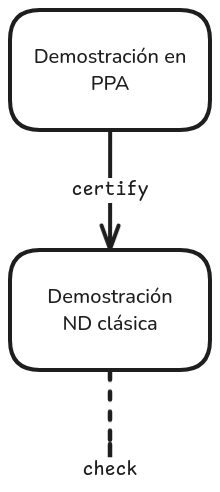
\includegraphics[scale=0.32]{img/ppt/certify.png}
                \centering
                \title{Arquitectura del certificador}
            \end{figure}
        \end{column}
    \end{columns}

    \begin{block}{Criterio de de Bruijn}
        Un asistente de demostración cumple con el criterio de de Bruijn si
        satisface que sus demostraciones puedan ser chequeadas por un programa
        independiente, pequeño y confiable.
    \end{block}
\end{frame}

\begin{frame}{Contexto global}
    Se generan $N$ demostraciones de deducción natural para cada programa, y se guardan en el \textit{contexto global}. El chequeo se extiende a contextos.
    
    \begin{figure}
        \begin{columns}
            \begin{column}{0.4\textwidth}
                \begin{tabular}{c}
                    \lstinputlisting{listings/certifier/two-theorems.ppa}
                \end{tabular}
            \end{column}
            \begin{column}{0.3\textwidth}
                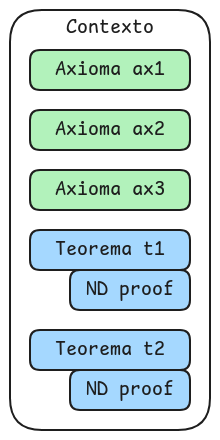
\includegraphics[scale=0.4]{img/ppa-context.png}
            \end{column}
        \end{columns}
        \caption{Contexto resultante de certificar un programa}
    \end{figure}
\end{frame}

\begin{frame}{Certificado de demostraciones}
    El certificado de una demostración es recursivo: se certifica cada comando, generando una demostración en deducción natural cuyas premisas son el certificado del resto de la demostración en PPA.
    \begin{figure}
        \begin{columns}
            \begin{column}{0.45\textwidth}
                \begin{tabular}{c}
                    \lstinputlisting{listings/ppt/certificado.ppa}
                \end{tabular}
    
            \end{column}
            \begin{column}{0.35\textwidth}
                \begin{prooftree}
                    \AxiomC{}
                    \RL{\alert{\ruleAxh{h}}}
                    \UnaryInfC{$h: p(v) \judG p(v)$}
                    \RL{\ruleExistsI}
                    \UnaryInfC{$h: p(v) \judG \exists x . p(X)$}
                    \RL{\ruleImpIh{h}}
                    \UnaryInfC{$\judG p(v) \fImp \exists x . p(X)$}
                \end{prooftree}
    
            \end{column}
        \end{columns}
        \caption{Ejemplo de certificado generado para un programa}
    \end{figure}
\end{frame}

\begin{frame}{Contexto local}
    Cada demostración tiene un contexto local a ella con las hipótesis agregadas por ciertos comandos (\lstinline{suppose}, \lstinline{consider}, \lstinline{have}, \lstinline{claim}, etc.). Necesaria para obtener las fórmulas asociadas a las hipótesis en el \lstinline{by}.

    \begin{figure}[h]
        \centering
        \begin{columns}
            \begin{column}{0.5\textwidth}
                \begin{tabular}{c}
                    \lstinputlisting{listings/certifier/local-context.ppa}
                \end{tabular}
            \end{column}
            \begin{column}{0.35\textwidth}
                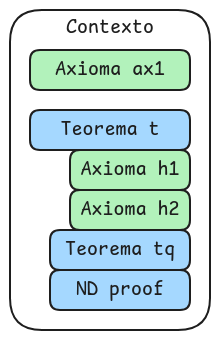
\includegraphics[scale=0.33]{img/ppa-local-context.png}
            \end{column}
        \end{columns}
        \caption{Ejemplo de contexto local}
    \end{figure}
\end{frame}

\begin{frame}{Certificado del by}
    Teniendo $\ctx = \{\hypId_1: \formTwo_1, \dots, \hypId_n: \formTwo_n\}$, para certificar \lstinline{thus A by h1, ..., hn}:

    \begin{enumerate}
        \item Buscamos las hipótesis en el contexto. Queremos demostrar
        \[
            \formTwo_1 \fAnd \dots \fAnd \formTwo_n \fImp \form
        \]
        \item \textbf{Razonamos por el absurdo}: Asumiendo la negación buscamos una contradicción
        \begin{align*}
            \fNot (\formTwo_1 \fAnd \dots \fAnd \formTwo_n \fImp \form)
            &\equiv \fNot (\fNot (\formTwo_1 \fAnd \dots \fAnd \formTwo_n) \fOr \form)\\
            &\equiv \formTwo_1 \fAnd \dots \fAnd \formTwo_n \fAnd \fNot \form
        \end{align*}
        \item Convertimos la negación a forma normal disyuntiva (\textbf{DNF})
        \[
            (\formLit_{1} \fAnd \dots \fAnd \formLit_n)
            \fOr \dots \fOr
            (\formLitTwo_{1} \fAnd \dots \fAnd \formLitTwo_m)
        \]
        \item Buscamos una \textbf{contradicción} refutando cada cláusula individualmente. Será refutable si
        \begin{itemize}
            \item Contiene $\fFalse$ o dos fórmulas opuestas ($\formLit, \fNot \formLit$), 
            \item Eliminando existenciales consecutivos y reiniciando el proceso, se consigue una refutación ($\fNot \pred(k), \forall \var . \pred(\var)$)
        \end{itemize}
    \end{enumerate}
\end{frame}

\begin{frame}{Ejemplo sin cuantificadores (1/2)}
    Tenemos el siguiente programa

    \begin{figure}[H]
        \centering
        \begin{tabular}{c}
            \lstinputlisting{listings/certifier/by-modus-ponens.ppa}
        \end{tabular}
    \end{figure}
    \begin{enumerate}
        \item Para certificar \lstinline{thus b by ax1, ax2} hay que generar una
        demostración para la implicación \[\big((a \fImp b) \wedge a \big)\fImp b\]
        \item Negamos la fórmula 
        \[ \fNot [ \big( (a \to b) \fAnd a \big) \to b ] \]
    \end{enumerate}
\end{frame}
\begin{frame}{Ejemplo sin cuantificadores (2/2)}
    \begin{enumerate}
        \setcounter{enumi}{2}
        \item La convertimos a DNF
        \begin{align*}
            &\fNot [ \big( (a \to b) \fAnd a \big) \to b ] \\
            &\equiv \fNot [ \fNot \big( (a \to b) \fAnd a \big) \fOr b ]
                && \just{\form \to \formTwo \equiv \fNot \form \fOr \formTwo}\\
            &\equiv \fNot \fNot \big( (a \to b) \fAnd a \big) \fAnd \fNot b
                && \just{\fNot(\form \fOr \formTwo) \equiv \fNot \form \fAnd \fNot \formTwo}\\
            &\equiv \big( (a \to b) \fAnd a \big) \fAnd \fNot b
                && \just{\fNot\fNot \form \equiv \form}\\
            &\equiv (\fNot a \fOr b) \fAnd a \fAnd \fNot b
                 && \just{\form \to \formTwo \equiv \fNot \form \fOr \formTwo}\\
            &\equiv (\fNot a \fOr b) \fAnd a \fAnd \fNot b
                && \just{(\form \fOr \formTwo) \fAnd \formThree \equiv (\form \fAnd \formThree) \fOr (\formTwo \fAnd \formThree)}\\
            &\equiv \begin{aligned}[t]
                &(\fNot a \fAnd a \fAnd \fNot b)\ \vee\\
                &(b \fAnd a \fAnd \fNot b)
            \end{aligned}
        \end{align*}
        \item Refutamos cada cláusula
        \[
            (\alert{\fNot a} \fAnd \alert{a} \fAnd \fNot b) \vee
            (\alert{b} \fAnd a \fAnd \alert{\fNot b})
        \]
    \end{enumerate}
\end{frame}

\begin{frame}{Ejemplo con cuantificadores (1/3)}
    Tenemos el siguiente programa

    \begin{figure}[H]
        \centering
        \begin{tabular}{c}
            \lstinputlisting{listings/certifier/by-modus-ponens-quant.ppa}
        \end{tabular}
    \end{figure}

    \begin{enumerate}
        \item Para certificar \lstinline{thus q(a) by ax1, ax2} hay que generar una
        demostración para la implicación \[
            \Big(\big(\forall x. (p(x) \fImp q(x))\big) \fAnd p(a) \Big)
            \fImp q(a)
        \]
        \item Negamos la fórmula 
        \[
            \fNot \left[
            \Big(\big(\forall x. (p(x) \fImp q(x))\big) \fAnd p(a) \Big)
            \fImp q(a)
        \right]
        \]
    \end{enumerate}
\end{frame}

\begin{frame}{Ejemplo con cuantificadores (2/3)}
    \begin{enumerate}
        \setcounter{enumi}{2}
        \item La convertimos a DNF
        \begin{align*}
            &\fNot \left[
                \Big(\big(\forall x. (p(x) \fImp q(x))\big) \fAnd p(a) \Big)
                \fImp q(a)
            \right] \\
            &\equiv \fNot \left[
                \fNot \Big(\big(\forall x. (p(x) \fImp q(x))\big) \fAnd p(a) \Big)
                \fOr q(a)
            \right] \\
            &\equiv
                \fNot \fNot \Big(\big(\forall x. (p(x) \fImp q(x))\big) \fAnd p(a) \Big)
                \fAnd \fNot q(a)\\
            &\equiv \big(\forall x. (p(x) \fImp q(x))\big) \fAnd p(a)
            \fAnd \fNot q(a)
        \end{align*}

        como a los ojos de DNF un $\forall$ es opaco, a pesar de que dentro
        tenga una implicación, la fórmula ya está en forma normal.

        \item Buscamos una contradicción refutando cada cláusula. No hay forma
        encontrando literales opuestos o $\fFalse$, por ej. la cláusula
        $p(a)$ no es refutable.
    \end{enumerate}
\end{frame}

\begin{frame}{Ejemplo con cuantificadores (3/3)}
    \begin{enumerate}
        \setcounter{enumi}{4}
        \item Probamos eliminando $\forall x. (p(x) \fImp q(x))$. Reemplazamos
        $x$ por una meta-variable fresca $\metavar{u}$.
        \[
            (p(\metavar{u}) \fImp q(\metavar{u})) \fAnd p(a) \fAnd \fNot q(a)
        \]
        \item Convertimos a DNF
        \begin{align*}
            &(p(\metavar{u}) \fImp q(\metavar{u})) \fAnd p(a) \fAnd \fNot q(a)\\
            &\equiv (\fNot p(\metavar{u}) \fOr q(\metavar{u})) \fAnd p(a) \fAnd \fNot q(a)\\
            &\equiv ( (\fNot p(\metavar{u}) \fAnd p(a)) \fOr (q(\metavar{u}) \fAnd p(a))) \fAnd \fNot q(a)\\
            &\equiv 
            \begin{aligned}[t]
                &(\fNot p(\metavar{u}) \fAnd p(a) \fAnd \fNot q(a))\ \fOr\\
                &(q(\metavar{u}) \fAnd p(a)\fAnd \fNot q(a))
            \end{aligned}
        \end{align*}
        \item Buscamos una contradicción refutando cada cláusula. Los
        literales opuestos tienen que \textit{unificar} en lugar de ser iguales.
        \begin{itemize}
            \item $\alert{\fNot p(\metavar{u})} \fAnd \alert{p(a)} \fAnd \fNot q(a)$ tenemos $p(\metavar{u}) \unify p(a)$ con $\subst{\metavar{u}}{a}$
            \item $\alert{q(\metavar{u})} \fAnd p(a) \fAnd \alert{\fNot q(a)}$ tenemos $q(\metavar{u}) \unify q(a)$ con $\subst{\metavar{u}}{a}$
        \end{itemize}
    \end{enumerate}
\end{frame}

\begin{frame}{Deducción natural}
    \begin{alertblock}{Desafío}
        ¡Hay que generar una demostración en deducción natural!
    \end{alertblock}

    Pasos

    \begin{itemize}
        \item \textbf{Razonamiento por el absurdo}: mediante las \textit{reglas admisibles} cut y eliminación de la doble negación (\ruleDnegE).
        \item \textbf{Conversión a DNF}: mediante la implementación de un \textit{sistema de reescritura}.
        \item \textbf{Contradicciones}: mediante la \textit{regla admisible} \ruleAndEProj{\anyForm} + \ruleOrE{} + \ruleNotI{}.
        \item \textbf{Eliminación de cuantificadores universales}: mediante unificación y \ruleForallE{}.
    \end{itemize}
\end{frame}

\begin{frame}{Razonamiento por el absurdo}
    \[
        \judG \formTwo_1 \fAnd \dots \fAnd \formTwo_n \fImp \form
        \overset{?}{\rightsquigarrow}
        \fNot (\formTwo_1 \fAnd \dots \fAnd \formTwo_n \fImp \form) \judG \fFalse
    \]
    \begin{columns}
        \begin{column}{0.4\textwidth}
            \begin{theorem}[DNeg Elim]
                \begin{prooftree}
                    \AxiomC{}
                    \RL{\ruleDnegE}
                    \admissibleRuleLine
                    \UnaryInfC{$\fNot \fNot \form \judG \form$}
                \end{prooftree}
            \end{theorem}        
        \end{column}
        % "Cortar el flujo de la demostración"
        \begin{column}{0.4\textwidth}
            \begin{theorem}[cut]
                \begin{prooftree}
                    \AxiomC{$\ctx, \formTwo \judG \form$}
                    \AxiomC{$\ctx \judG \formTwo$}
                    \RL{\ruleCut}
                    \admissibleRuleLine
                    \BinaryInfC{$\ctx \judG \form$}
                \end{prooftree}
            \end{theorem}
        \end{column}
    \end{columns}
    \begin{lemma}[Razonamiento por el absurdo]
        \begin{prooftree}
            \AxiomC{$\vdots$}
            \noLine
            \UnaryInfC{$\ctx, \fNot \form \judG \fFalse$}
            \RL{\ruleNotI}
            \UnaryInfC{$\ctx \judG \fNot\fNot \form$}
            \RL{\ruleCutWith{\ruleDnegE}}
            \admissibleRuleLine
            \UnaryInfC{$\ctx \judG \form$}
        \end{prooftree}
        \vspace{0.1cm}
    \end{lemma}
    
\end{frame}

\begin{frame}{Conversión a DNF}
    Implementamos una traducción mediante el siguiente sistema de reescritura. \textbf{Algoritmo}: reescribir de a un paso hasta que no cambie (clausura de Kleene)
        \begin{align*}
            \fNot\fNot \formLit &\rewrite
                \formLit
                &&\text{eliminación de $\fNot\fNot$}\\
            \fNot \fFalse &\rewrite
                \fTrue\\
            \fNot \fTrue &\rewrite
                \fFalse\\
            \formLit \fImp \formLitTwo &\rewrite
                \fNot \formLit \fOr \formLitTwo
                &&\text{definición de implicación}\\
            \fNot(\formLit \fOr \formLitTwo) &\rewrite
                \fNot \formLit \fAnd \fNot \formLitTwo
                &&\text{distributiva de $\fNot$ sobre $\fAnd$}\\
            \fNot(\formLit \fAnd \formLitTwo) &\rewrite
                \fNot \formLit \fOr \fNot \formLitTwo
                &&\text{distributiva de $\fNot$ sobre $\fOr$}\\
            (\formLit \fOr \formLitTwo) \fAnd \formLitThree &\rewrite
                (\formLit \fAnd \formLitThree) \fOr (\formLitTwo \fAnd \formLitThree)
                &&\text{distributiva de $\fAnd$ sobre $\fOr$ (der)}\\
            \formLitThree \fAnd (\formLit \fOr \formLitTwo) &\rewrite
                (\formLitThree \fAnd \formLit) \fOr (\formLitThree \fAnd \formLitTwo)
                &&\text{distributiva de $\fAnd$ sobre $\fOr$ (izq)}\\
            \formLit \fOr (\formLitTwo \fOr \formLitThree) &\rewrite
                (\formLit \fOr \formLitTwo) \fOr \formLitThree
                &&\text{asociatividad de $\fOr$}\\
            \formLit \fAnd (\formLitTwo \fAnd \formLitThree) &\rewrite
                (\formLit \fAnd \formLitTwo) \fAnd \formLitThree
                &&\text{asociatividad de $\fAnd$}
        \end{align*}
\end{frame}

\begin{frame}{Conversión a DNF - Congruencias}
    Para reescribir una sub-fórmula (trivial sintácticamente), hay que demostrar las congruencias de los conectivos.
    \[
        \formLit \fOr \alert{\fNot (\formLitTwo \fOr \formLitThree)}
        \rewrite
        \formLit \fOr \alert{(\fNot \formLitTwo \fAnd \fNot \formLitThree)}
    \]

    \begin{block}{Congruencias}
        \begin{align*}
            \form \judG \form'
                &\Rightarrow \form \fAnd \formTwo \judG \form' \fAnd \formTwo\\
            \form \judG \form'
                &\Rightarrow \form \fOr \formTwo \judG \form' \fOr \formTwo\\
            \form' \judG \form
                &\Rightarrow \fNot \form \judG \fNot \form'
        \end{align*}        
    \end{block}

    \begin{alertblock}{$\fNot$ es contravariante}
        Para demostrar $\fNot \form \judG \fNot \form'$ no necesitamos una demostración de $\form \judG \form'$, sino de $\form' \judG \form$.
        
        $\Rightarrow$ para todas las reescrituras, incluso las congruencias, tenemos que demostrarlas en ambos sentidos.
    \end{alertblock}
\end{frame}

\begin{frame}{Conversión a DNF - Reglas admisibles}
    \begin{block}{Reglas admisibles para conversión a DNF}
        \begin{columns}[t]
        \begin{column}{0.5\textwidth}
            \centering
            Pasos base
            \begin{align*}
            \fNot\fNot \formLit &\judgEquiv
                \formLit
                \\
            \fNot \fFalse &\judgEquiv
                \fTrue\\
            \fNot \fTrue &\judgEquiv
                \fFalse\\
            \formLit \fImp \formLitTwo &\judgEquiv
                \fNot \formLit \fOr \formLitTwo
                \\
            \fNot(\formLit \fOr \formLitTwo) &\judgEquiv
                \fNot \formLit \fAnd \fNot \formLitTwo
                \\
            \fNot(\formLit \fAnd \formLitTwo) &\judgEquiv
                \fNot \formLit \fOr \fNot \formLitTwo
                \\
            (\formLit \fOr \formLitTwo) \fAnd \formLitThree &\judgEquiv
                (\formLit \fAnd \formLitThree) \fOr (\formLitTwo \fAnd \formLitThree)
                \\
            \formLitThree \fAnd (\formLit \fOr \formLitTwo) &\judgEquiv
                (\formLitThree \fAnd \formLit) \fOr (\formLitThree \fAnd \formLitTwo)
                \\
            \formLit \fOr (\formLitTwo \fOr \formLitThree) &\judgEquiv
                (\formLit \fOr \formLitTwo) \fOr \formLitThree
                \\
            \formLit \fAnd (\formLitTwo \fAnd \formLitThree) &\judgEquiv
                (\formLit \fAnd \formLitTwo) \fAnd \formLitThree
            \end{align*}
        \end{column}
        \begin{column}{0.5\textwidth}
            \centering
            Pasos recursivos de congruencia
            
            (con $\form \judgEquiv \form'$)
            \begin{align*}
                \form \fAnd \formTwo &\judgEquiv \form' \fAnd \formTwo\\
                \form \fOr \formTwo &\judgEquiv \form' \fOr \formTwo\\
                \fNot \form &\judgEquiv \fNot \form'
            \end{align*}
        \end{column}
        \end{columns}
    \end{block}
\end{frame}

\begin{frame}{Contradicciones}
    \begin{exampleblock}{Ejemplo}
    \begin{prooftree}
        \def\defaultHypSeparation{\hskip .1in}
        \AxiomC{}
        \LL{\ruleAx}
        \UnaryInfC{\(
            \ctx \judG
            \begin{aligned}[b]
                &(\fNot a \fAnd a \fAnd \fNot b)\\
                &\vee (b \fAnd a \fAnd \fFalse)
            \end{aligned}
        \)}
        \AxiomC{$\someProof_L$}
        \noLine
        \UnaryInfC{\(
            \ctx, \fNot a \fAnd a \fAnd \fNot b \judG \fFalse
        \)}
        \AxiomC{}
        \RL{\ruleAx}
        \UnaryInfC{$\ctx_1 \judG b \fAnd a \fAnd \fFalse$}
        \RL{\ruleAndEProj{\fFalse}}
        \admissibleRuleLine
        \UnaryInfC{\(
            \ctx, b \fAnd a \fAnd \fFalse \judG \fFalse
        \)}
        \RL{\ruleOrE}
        \TrinaryInfC{\(
            \ctx = (\fNot a \fAnd a \fAnd \fNot b)
            \vee
            (b \fAnd a \fAnd \fFalse)
            \judG
            \fFalse
        \)}
    \end{prooftree}
    
    donde
    
    \begin{prooftree}
        \AxiomC{}
        \RL{\ruleAx}
        \UnaryInfC{$\ctx_1 \judG \fNot a \fAnd a \fAnd \fNot b$}
        \RL{\ruleAndEProj{\fNot a}}
        \admissibleRuleLine
        \UnaryInfC{$\ctx_1 \judG \fNot a$}
        \AxiomC{}
        \RL{\ruleAx}
        \UnaryInfC{$\ctx_1 \judG \fNot a \fAnd a \fAnd \fNot b$}
        \RL{\ruleAndEProj{a}}
        \admissibleRuleLine
        \UnaryInfC{$\ctx_1 \judG a$}
        \RL{\ruleNotE}
        \LL{$\someProof_L=$}
        \BinaryInfC{\(
            \ctx_1 = \ctx, b \fAnd a \fAnd \fFalse \judG \fFalse
        \)}
    \end{prooftree}
    \end{exampleblock}

    \begin{lemma}[Regla admisible \ruleAndEProj{\anyForm}]
        \begin{prooftree}
            \AxiomC{$\ctx \judG \anyForm_1 \fAnd \dots \fAnd \anyForm_i \fAnd \dots \fAnd \anyForm_n$}
            \AxiomC{$n \in \setNaturals$}
            \admissibleRuleLine
            \RL{\ruleAndEProj{\anyForm_{i}}}
            \BinaryInfC{$\ctx \judG \anyForm_i$}
        \end{prooftree}
    \end{lemma}
\end{frame}

\begin{frame}[fragile]{Alcance y limitaciones del by}
    \begin{itemize}
        \item \textbf{Completo} para lógica proposicional y \textbf{heurístico} para primer orden.
        \item Esto es aceptable, la validez de LPO es indecidible (Teorema de Church).
        \item Elimina los $\forall$ consecutivos de a lo sumo una hipótesis. Pero le faltan más cosas.
    \end{itemize}
\begin{figure}
    \centering
    \small Ejemplo de falla en eliminación
    \vspace{0.1cm}

    \begin{tabular}{c}
\begin{lstlisting}
axiom ax1: forall X . p(X) -> q(X)
axiom ax2: forall X . p(X)
theorem t: q(a)
proof
    thus q(a) by ax1, ax2
end
\end{lstlisting}
    \end{tabular}
\end{figure}
\end{frame}

% Considerar saltear esto si no da el tiempo
\begin{frame}{Descarga de conjunciones}
    \todo{Agregar esto}
\end{frame}

\section{Extracción de testigos}




\end{document}